\section{Methods \label{chapter2}}
\subsection{Noise Design}
\textsc{NMF} is expected to be rubost to various noises. Robust algorithms has to successfully reduce the amount of noise while preserving the edges and has no blurring effect on the image (\citet{barbu2013variational}). Here we design three kinds of noises, i.e. Gaussian noise, Poisson noise, and Salt \& Pepper noise. \newline 
\textbf{Gaussian noise} is a statistical noise having a probability density function equal to that of the normal distribution. \textbf{Poisson noise} or shot noise is a type of electronic noise that
occurs when the finite number of particles that carry energy,
such as electrons in an electronic circuit or photons in an optical
device, is small enough to give rise to detectable statistical
fluctuations in a measurement. An image containing \textbf{Salt \& Pepper noise} noise will have dark pixels
in bright regions and bright pixels in dark regions (\citet{sampat2005computer}).
\begin{figure}[h]
	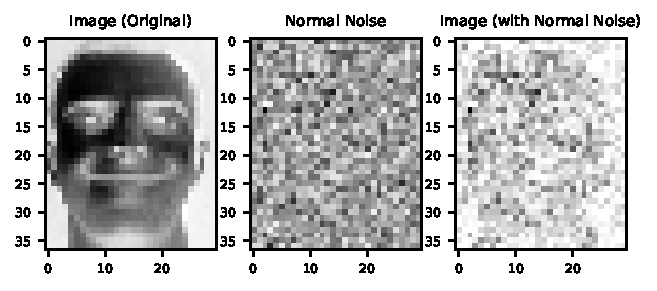
\includegraphics[width=4.5cm, height=3cm]{Noise_ORL_Normal_Comparison.pdf}
	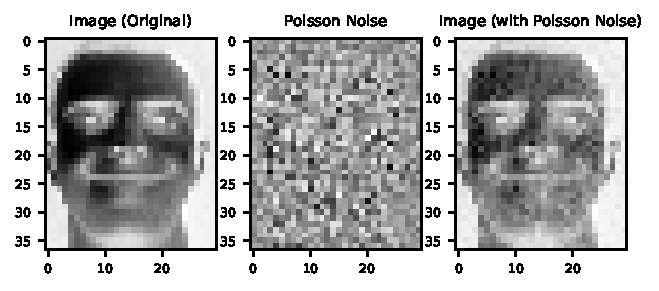
\includegraphics[width=4.5cm, height=3cm]{Noise_ORL_Poisson_Comparison.pdf}
	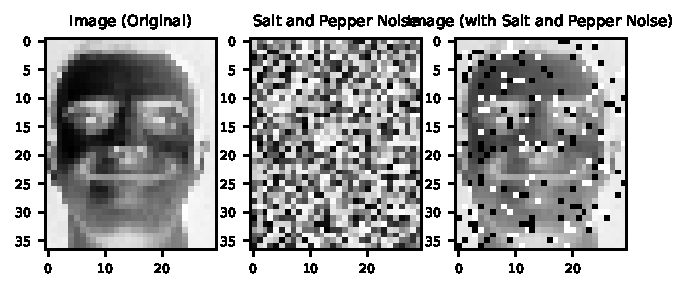
\includegraphics[width=4.5cm, height=3cm]{Noise_ORL_Salt_and_Pepper_Comparison.pdf}
	\caption{Illustration of Gaussian Noise, Poisson Noise, and Salt \& Pepper Noise}
	\label{fig:noise}
\end{figure}
\subsection{NMF and Gaussian noise}
\citet{lee2001algorithms} propose the first \textsc{nmf} with the objective function between imaga~$V$ and its \textsc{nmf} factorisation~$W$ and~$H$ being
\begin{equation*}
  \left\Vert V-WH \right\Vert= \sum_{ij} \left[V_{ij}-(WH)_{ij}\right]^2.
\end{equation*}
To minimise this object function of least square, \citet{lee2001algorithms} prove the convergence of the multiplication update rule
\begin{equation*}
H_{jk}\leftarrow H_{jk}\frac{(W^{T}V)_{jk}}{(W^{T}WH)_{jk}} \text{ and } W_{ij}\leftarrow W_{ij}\frac{(VH)_{ij}}{(WHH^{T})_{ij}}.
\end{equation*}
Here, $()_{ij}/()_{ij}$ denotes elementwise division of the two matrix. \citet{liu2015performance} shows this \textsc{nmf} algorithm minimises Gaussian.

\subsection{KLNMF and Poisson noise}
\citet{lee2001algorithms} suggest that \textsc{klnmf} is a algorithm that minimising the Kullback-Leibler divergence
\begin{eqnarray}
  D(V||WH)&=&\sum_{ij}\left(V_{ij}\log\frac{V_{ij}}{\left(WH\right)_{ij}}-V_{ij}+\left(WH\right)_{ij}\right)\nonumber\\
          &=&\sum_{ij}\left(-V_{ij}\log\left(WH\right)_{ij}+\left(WH\right)_{ij}+C(V_{ij})\right).\label{eq:klobj}
\end{eqnarray}
where $C(V_{ij})=V_{ij}\log V_{ij}-V_{ij}$. $C(V_{ij})$ is a function of the observed image matrix~$V$ only.
\citet{lee2001algorithms} also suggest a multiplication update rule to find as the optimisation procedure of \textsc{klnmf}
\begin{equation*}
H_{jk}\leftarrow H_{jk}\frac{\sum_{i}W_{ij}V_{ik}/(WH)_{jk}}{\sum_{i'}W_{i'j}} \text{ and } W_{ij}\leftarrow W_{ij}\frac{\sum_{k}H_{jk}V_{ik}/(WH)_{jk}}{\sum_{k'}H_{ik'}}.
\end{equation*}
As this original image matrix~$V$ is observed, minimising this Kullback-Leibler divergence~\eqref{eq:klobj} is equivalent to minimising
\begin{equation*}
  \sum_{ij}\left(-V_{ij}\log\left(WH\right)_{ij}+\left(WH\right)_{ij}+C(V_{ij})\right).
\end{equation*},
for arbitrary bounded function~$C(V_{ij})$. Taking exponential of the negative of this score function, the problem transforms to maximising the following likelihood function
\begin{equation*}
L(WH|V)=\prod_{ij}\left(\left(WH\right)_{ij}^{V_{ij}}e^{-\left(WH\right)_{ij}}+C(V_{ij})\right).
\end{equation*}
Choosing constant $C(V_{ij})$ to be $-\log V_{ij}!$ gives
\begin{equation*}
L(WH|V)=\prod_{ij}\left(\frac{\left(WH\right)_{ij}^{V_{ij}}e^{-\left(WH\right)_{ij}}}{V_{ij}!}\right).
\end{equation*}
Hence, the probability density function of each element of the original matrix~V is Poisson
\begin{equation*}
P(V_{ij})=\frac{\left(WH\right)_{ij}^{V_{ij}}e^{-\left(WH\right)_{ij}}}{V_{ij}!}
\end{equation*}
is a sufficient condition to yield this likelihood. Hence \textsc{klnmf} is most suitable for images with Poisson noise.
\subsection{Asymptotic equivalence of noise distributions}
 We design an Gaussian noise and a Poisson noise with different magnitude.
 Poisson distribution with parameter~$\lambda$ (integer) is equivalent to the sum of $\lambda$ Poisson distributions with parameter~$1$ \citep[][p. 45]{Walck:1996cca}.
 Hence for $\lambda$ large, Central Limit Theorem implies that Poisson distribution with parameter~$\lambda$ is well approximated by $N(\lambda,\lambda)$.
 When applying Poisson noise to an image, we do not degree of freedom to choose any parameter.
 The variance is the magnitude of the pixels. To compare the robustness of \textsc{klnmf} with \textsc{nmf} with different noise, we choose the variance of Gaussian noise to be the different from the magnitude of the pixel, that is, $N(0,\operatorname{Var})\neq N(0,V)\approx \operatorname{Poi}(V)-V$.
 Figure~\ref{noise} visualises the similarity of Poisson distribution and Normal distribution with parameter~$V=40$.
\begin{figure}
  \centering
  % Requires \usepackage{graphicx}
  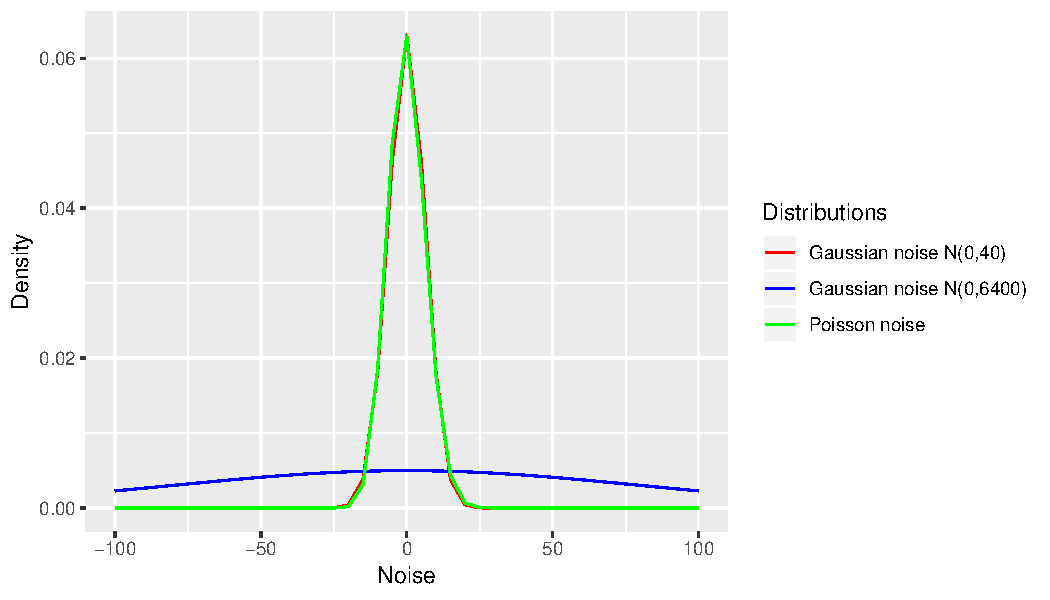
\includegraphics[scale=1]{resource/noise}\\
  \caption{Compare a Gaussian noise~$N(0,40)$ with Poisson noise $\operatorname{Poi}(40)-40$. They two distributions are asymptotically equivalent and have similar density functions.}\label{noise}
\end{figure}

\csvautobooktabular{{"../results/statistics".csv}}
\subsection{Preprocessing}
We apply global centring and local centring to preprocess the image data~\texttt{Vhat}
\begin{lstlisting}[caption=Centring image data, label=matn1]
n_samples = len(Vhat)
# global centering
Vhat = Vhat - Vhat.mean(axis=0)
# local centering
Vhat -= Vhat.mean(axis=1).reshape(n_samples, -1)
Vhat -= Vhat.min()
\end{lstlisting}
